%==============================================================================
%  Zr3d Code Architecture
%
%  Standalone. No external figures: the flowchart of Section 4 is TikZ.
%  Compiles with pdflatex; also fine on Overleaf.
%==============================================================================
\documentclass[11pt]{article}

\usepackage[margin=1in]{geometry}
\usepackage{amsmath,amssymb}
\usepackage{booktabs}
\usepackage{longtable}
\usepackage{array}
\usepackage{graphicx}
\usepackage{xcolor}
\usepackage{listings}
\usepackage{hyperref}
\usepackage{tikz}
\usetikzlibrary{arrows.meta,positioning,fit,backgrounds,calc,shapes.geometric}

\hypersetup{colorlinks=true,linkcolor=blue!50!black,urlcolor=blue!50!black,
            citecolor=blue!50!black}

\setcounter{secnumdepth}{4}
\setcounter{tocdepth}{3}

% ---- shorthands -------------------------------------------------------------
\newcommand{\aloop}{\ensuremath{\langle a\rangle}}
\newcommand{\cloop}{\ensuremath{\langle c\rangle}}
\newcommand{\ZrM}{\textsf{ZrMicro}}
\newcommand{\MoD}{\textsf{MoDELib3}}
\newcommand{\MoDfull}{\textsf{MoDELib-fullCD}}
\newcommand{\MoDnnl}{\textsf{MoDELib2-NNL}}
\newcommand{\Zrd}{\textsf{Zr3d\_ghoniem}}
\newcommand{\code}[1]{\texttt{\small #1}}
\newcommand{\file}[1]{\texttt{\footnotesize #1}}

% Equation references into the deliverable
\newcommand{\dref}[1]{Eq.~(#1)}
\newcommand{\drefs}[2]{Eqs.~(#1)--(#2)}

\lstset{basicstyle=\ttfamily\footnotesize,
        breaklines=true,
        columns=fullflexible,
        frame=single,
        framesep=4pt,
        rulecolor=\color{black!30},
        backgroundcolor=\color{black!3},
        showstringspaces=false}

% ---- flowchart palette ------------------------------------------------------
\definecolor{cNotebook}{RGB}{ 33, 87,150}   % orchestration
\definecolor{cPy}      {RGB}{ 45,125, 90}   % ZrMicro python
\definecolor{cCpp}     {RGB}{155, 60, 30}   % ZrMicro C++
\definecolor{cMod}     {RGB}{110, 55,140}   % MoDELib C++
\definecolor{cData}    {RGB}{140,110, 20}   % files on disk
\definecolor{cOut}     {RGB}{ 70, 70, 70}   % products

\title{\textbf{Zr3d Code Architecture}}
\author{Nasr M. Ghoniem}
\date{\today}

\begin{document}
\maketitle

\begin{abstract}
\noindent
This document describes the architecture of the \Zrd{} code: the software that
solves the spatially-resolved cluster-dynamics (SR-CD) model of irradiated
zirconium, and the zero-dimensional \ZrM{} model against which it is verified.
The code is not a single program. It is a two-repository system driven from a
Jupyter notebook, in which a Python orchestration layer, a C++ stiff-ODE
integrator, and a C++ finite-element field solver each own one part of the
problem and exchange state through well-defined interfaces. Section~\ref{sec:arch}
describes the workflow, Section~\ref{sec:components} enumerates the components and
their locations, Section~\ref{sec:input} lists the inputs with typical values and
units, Section~\ref{sec:flow} gives the call graph, and Section~\ref{sec:classes}
documents the classes and data structures with references to the governing
equations of the Phase-4 D1/M1 deliverable
(\file{Docs/Formulation/GW\_Phase4\_D1M1\_NG.pdf}, cited throughout as
\dref{n}). Sections~\ref{sec:arch}--\ref{sec:classes} describe \Zrd{} as it now
stands; Section~\ref{sec:changes} then separates what was inherited from the
original \MoD{} from what was added, at the level of both the equations and the
input data. Appendix~\ref{sec:manual} is the operating manual.
\end{abstract}

\tableofcontents

%==============================================================================
\section{General Architecture}
\label{sec:arch}

\subsection{The problem the architecture has to solve}

The physics splits cleanly into two time scales, and the architecture is a direct
expression of that split.

The \emph{mobile} species --- vacancies, single interstitials, di- and
tri-interstitials --- relax to their local sink field in of order milliseconds.
The \emph{immobile} species --- the four loop families --- evolve over dose
steps of order $10^{7}$~s. The ratio is $\sim 10^{10}$. Integrating both with one
time integrator would be wasteful at best and intractable at worst.

The deliverable therefore poses the mobile species as a \emph{quasi-steady}
reaction--diffusion boundary-value problem with no time-derivative term at all,
\dref{1},
\begin{equation}
0 = -\nabla\!\cdot\!\boldsymbol{J} + P_M
    + \tfrac{1}{2}\,\boldsymbol{c}_M^{T} R_2\,\boldsymbol{c}_M
    + (E-D)\,\boldsymbol{c}_M + S_{vL},
\label{eq:mobile}
\end{equation}
and marches the immobile species pointwise in dose against the frozen mobile
field, \dref{34} for the density and \dref{39} for the content. This is an
operator-split quasi-steady-state approximation (QSSA): within one dose step the
fast manifold is solved to steady state, then the slow manifold is advanced with
the fast one held fixed.

\subsection{Two execution routes}

That split can be realized in two ways, and \emph{both exist in this codebase}.
They share the material definitions and the physics, but not the driver. Confusing
them is the single most common source of misinterpretation, so they are separated
explicitly here.

\paragraph*{Route A --- notebook-driven coupled march.}
Driven by \file{ZrMicro/code/coupled\_0d\_3d\_ZrMicro.ipynb}. Python owns the
dose loop. Within each step it calls \MoD{} to solve the fast mobile BVP on the
finite-element mesh, then advances the slow immobile state \emph{using the \ZrM{}
C++ integrator} with the mobile species pinned
(\code{freeze\_mobile=1}), one OpenMP batch case per quadrature point. The
immobile physics executed here is \ZrM{}'s, evaluated at many spatial points.

\paragraph*{Route B --- monolithic \MoD{} run.}
Driven by \file{tutorials/zrmicro\_coupled/clean\_run.sh}, which invokes
\code{microstructureGenerator} and then \code{DDomp}. Everything happens inside
\MoD{}: \code{ClusterDynamicsFEM::solveMobileClusters()} performs the Newton
solve of Eq.~\eqref{eq:mobile}, and \code{solveImmobileClusters()} marches the
loop families node by node. No Python is involved at run time. This is the route
that produced the 30~dpa verification results, and it is the route the \Zrd{}
branch modifies.

\medskip
\noindent
Route A is the \emph{coupling harness}: it tests the splitting and lets the 0-D
physics be exercised in space. Route B is the \emph{3-D code proper}: it is where
the SR-CD equations of deliverable Sec.~2.2 are actually implemented. The
remainder of this document covers both, labelling each component by the route in
which it participates.

\subsection{The notebook workflow, cell by cell}

The notebook is the orchestrator for Route A and the entry point a user actually
touches. Its structure is linear and each stage has one responsibility.

\begin{enumerate}
\item \textbf{Formulation (markdown, cells 0--5).} The 3-D SR-CD model, the
reduced 0-D model, the correspondence between them, and the numerical methods.
No code; this is the specification the rest of the notebook implements.

\item \textbf{Bootstrap (cell 7).} Resolves \file{ZrMicro/} from the notebook
location --- tolerating launch from \file{code/}, from \file{ZrMicro/}, or from
the repository root --- puts it on \code{sys.path}, and imports the entire Python
layer: \code{InputData}, \code{ReactionRates}, \code{RateEquations},
\code{cpp\_bridge}, \code{post\_process}, \code{visualization},
\code{modelib\_coupling}, \code{modelib\_export}, \code{modelib\_fem}.

\item \textbf{Build management (cells 8--10).} Two independent builds are ensured
before anything runs.
\code{ensure\_zrmicro\_solver()} locates \code{solver.exe}, configuring and
building through CMake if absent.
\code{ensure\_modelib()} constructs a \code{MoDELibFEMSolver} and, if \code{DDomp}
is missing, runs the WSL build script. On Windows \MoD{} is built inside WSL and
its \code{DDomp} is a Linux ELF, so it is invoked through \code{wsl.exe} with
Windows paths translated to \file{/mnt/<drive>/...}.
\emph{Both build paths verify artifacts on disk rather than trusting exit status},
because the build script terminates in a \code{|| echo WARN} and returns zero
even when it produced nothing.

\item \textbf{User controls (cell 12).} One block holds every knob: the dose
schedule (\code{DOSE\_START}, \code{DOSE\_INTERVAL}, \code{DOSE\_MAX}), the
physical conditions ($T$, $G$, $\sigma_n$) applied to \emph{both} codes, the
spatial discretization, the runtime flags, the 0-D solver configuration, and the
fitted \code{PARAMETER\_OVERRIDES} set. The overrides are pinned at full
precision rather than inherited from the workbook, because the workbook has
drifted since the reference run: 28 parameters differ and 11 are now absent
from it entirely.

\item \textbf{Model construction (cell 13).} \code{InputData} reads the workbook;
each override is routed automatically to whichever sheet already defines the key;
\code{calculate\_derived\_parameters()} recomputes the derived quantities; then
\code{ReactionRates} and \code{RateEquations} are built on top. Finally
\code{collect\_solver\_args()} flattens the whole parameter set into the
\code{--key=value} command line the C++ integrator consumes.

\item \textbf{Consistency check (cell 14).} Parses \MoD{}'s material file and
compares it against the \ZrM{} conditions field by field --- dose rate, species
vector, and the four DAD capture efficiencies of \dref{15} against the 0-D
symmetric forms \drefs{63}{64}. It also reports where the two models are known
\emph{not} to correspond, so that a residual is not mistaken for a bug.

\item \textbf{Run directory (cell 16).} A timestamped, git-hash-tagged output
directory, so every figure and every number is traceable to a commit.

\item \textbf{0-D reference run (cells 18--20).} The full \ZrM{} integration,
used both as the physical reference and as the source of the initial immobile
state for the march.

\item \textbf{Spatial grid and backend selection (cells 22--23).} The grid is
built in units of the depletion length $\ell = 1/\sqrt{Z_N\rho_N}$, the domain
spanning \code{DOMAIN\_IN\_ELL} multiples of it. The fast-solve backend is then
chosen: \code{modelib} if \code{DDomp} is built \emph{and} the simulation
directory is seeded, otherwise an analytic \code{placeholder}
$C_M^{*}(x) = [1-e^{-x/\ell}]\,C_M^{\rm bulk}$. The placeholder is loudly
labelled as not being a FEM result --- it scales all four species by the same
factor, which cannot represent species-dependent depletion lengths that here
differ by four orders of magnitude.

\item \textbf{Operator-split march (cell 25).} The core loop, discussed below.

\item \textbf{Post-processing (cells 26--33).} Regression against the 0-D
reference, 3-D field plots, grain-boundary profiles, and a provenance manifest.
\end{enumerate}

\subsection{The dose march}

Stripped to its essentials, the march is:

\begin{lstlisting}
Y = [pack_y0(CM0[q], immobile_0, rho_seed) for q in range(N_POINTS)]

for n in range(len(DOSE_SNAPSHOTS) - 1):
    Qv = q_per_variant_from_state(Y)      # loops -> (N, r) per family
    CM = fast_solve_field(dose[n], Qv)    # FAST: MoDELib FEM mobile BVP
    for q in range(N_POINTS):
        Y[q][0:4] = CM[q]                 # inject frozen mobile field
    Y = march(Y, times[n], times[n+1])    # SLOW: ZrMicro batch, freeze_mobile=1
    history[dose[n+1]] = Y
\end{lstlisting}

Three properties of this loop are worth stating explicitly.

\textbf{The coupling is two-way but staggered.} The loop state sets the sink
field that the mobile solve sees (through \code{q\_per\_variant\_from\_state},
which reduces the loop populations to a number density and a mean radius per
family); the resulting mobile field then drives loop growth over the step. Neither
is solved simultaneously with the other.

\textbf{The immobile march is itself substepped.} \code{march()} divides the dose
step into intervals no longer than \code{MAX\_SUBSTEP\_S} and calls
\code{run\_immobile\_step} on each. A point that fails to integrate retains its
previous state and is reported rather than aborting the run.

\textbf{Every quadrature point is one batch case.} \code{run\_immobile\_step}
builds one \code{--key=value} case per point, all sharing the material parameters
in \code{base\_cli} (valid because $T$, $\sigma$ and the bias factors are
spatially uniform) and differing only in the initial state and the integration
window. They are integrated concurrently by the OpenMP batch mode of the C++
solver in a single subprocess. This is what makes the pointwise march affordable:
it amortizes the process-spawn cost, which dominates on Windows.

%==============================================================================
\section{Code Components}
\label{sec:components}

\subsection{Repositories}

The code spans the two repositories of Table~\ref{tab:repos}.

\begin{table}[htbp]
\centering
\caption{The two repositories.}
\label{tab:repos}
\begin{tabular}{@{}lll@{}}
\toprule
repository & remote & role \\
\midrule
\file{Fluor\_Zr} & \file{Ghoniem/Fluor\_Zr} &
  0-D model, orchestration, post-processing, documents \\
ile{MoDELib3} & ile{Ghoniem/MoDELib3}, branch ile{zr3d\_ghoniem} &
  3-D FEM SR-CD solver \\
\bottomrule
\end{tabular}
\end{table}

\noindent
The \MoD{} work lives on the branch \file{zr3d\_ghoniem} of a fork. The
cluster-dynamics upstream is \file{mlm335/MoDELib-fullCD}, \emph{not}
\file{mlm335/MoDELib2-NNL} --- see Section~\ref{sec:changes}. Po's original
material definition \file{Zr4.txt} is left untouched --- the reconciled
definition is the separate file \file{Zr3d\_ghoniem.txt}.

\subsection{Python components (\file{Fluor\_Zr/ZrMicro/py\_utils/})}

Table~\ref{tab:python} lists the Python layer. It carries no physics that the
C++ layer does not also carry: its role is to read the inputs, derive the
constants, orchestrate, and post-process.

\begin{longtable}{@{}p{0.26\textwidth}p{0.09\textwidth}p{0.57\textwidth}@{}}
\caption{Python layer. ``Route'' marks which execution route uses the module:
A = notebook coupled march, B = monolithic \MoD{} run, P = post-processing
common to both.}
\label{tab:python}\\
\toprule
module & route & role \\
\midrule
\endfirsthead
\toprule
module & route & role \\
\midrule
\endhead
\file{input\_data.py} & A &
  \code{InputData}: reads the three-sheet workbook, supplies defaults for missing
  entries, and computes every derived quantity --- jump frequencies, equilibrium
  concentrations, length scales, generation-rate partition, DAD bias factors. \\
\file{reaction\_rates.py} & A &
  \code{ReactionRates}: all pairwise reaction rates $R_{a,b}$, sink
  concentrations \dref{66}, loop absorption \drefs{83}{89}, thermal emission,
  nucleation, annealing, and coalescence. State is cached per ODE call. \\
\file{rate\_equations.py} & A &
  \code{RateEquations}: the 19-equation right-hand side, initial conditions,
  loop radii, strain rates, hardening. Mirrors the C++ RHS exactly. \\
\file{cpp\_bridge.py} & A &
  Flattens the parameter set into \code{--key=value} arguments, launches
  \code{solver.exe} (single or \code{--batch\_file} mode), parses stdout into a
  solution matrix. \\
\file{simulation.py} & A &
  \code{ZrMicroSimulation}: the SciPy LSODA fallback path and an interrupt
  guard. Retained as a reference implementation. \\
\file{modelib\_coupling.py} & A &
  The operator-split driver. \code{pack\_y0} assembles the length-19 state per
  point; \code{build\_immobile\_cases} sets \code{freeze\_mobile=1} and the step
  window; \code{run\_immobile\_step} runs the batch and unpacks it. \\
\file{modelib\_fem.py} & A &
  \code{MoDELibFEMSolver}: writes the loop state into \MoD{}'s microstructure
  inputs, invokes \code{DDomp} (through \code{wsl.exe} when required), and reads
  the mobile field back at the quadrature points. \\
\file{modelib\_export.py} & A &
  Maps the lumped 0-D loop families onto the three \aloop{} prismatic variants
  using the resolved-stress weights $w_k(\sigma)$ of \dref{36}. \\
\file{modelib\_fields.py} & B, P &
  Reads \file{evl/*.txt} and \file{evl/cdNodes.txt}; plane-cut field panels and
  loop-platelet overlays. \\
\file{modelib\_gb.py} & B, P &
  Grain-boundary profiles of density, content, size and mobile species. Loop
  diameters are formed from binned mean content and density, not by averaging
  nodal diameters. \\
\file{post\_process.py} & A, P &
  Derived macroscopic quantities: loop radii and densities in physical units,
  growth and creep strains, hardening, conservation diagnostics. \\
\file{visualization.py} & A, P &
  \code{ZrMicroVisualizer}: the figure suite, the run directory, and
  \file{provenance.md}. \\
\file{pre\_process.py} & A &
  Input-file resolution, setup validation, parameter-range warnings. \\
\file{fit\_cloops.py}, \file{fit\_vacancy\_loops.py},
\file{fit\_strain\_factors.py} & --- &
  Offline parameter identification against the experimental sheets. \\
\file{transport\_audit.py} & --- & Diagnostic harness. \\
\bottomrule
\end{longtable}

\subsection{C++ components}

Table~\ref{tab:cpp} lists the compiled layer. The two C++ codes are entirely
independent builds --- different toolchains, different libraries, no shared
headers --- and communicate only through the interfaces of
Sec.~\ref{sec:interfaces}. Entries marked \textbf{New in \Zrd{}} have no
counterpart in the original \MoD{}; Sec.~\ref{sec:changes} separates the
inherited code from the added code in full.

\begin{longtable}{@{}p{0.30\textwidth}p{0.09\textwidth}p{0.53\textwidth}@{}}
\caption{C++ layer across both repositories.}
\label{tab:cpp}\\
\toprule
file & route & role \\
\midrule
\endfirsthead
\toprule
file & route & role \\
\midrule
\endhead
\multicolumn{3}{@{}l}{\textbf{\file{Fluor\_Zr/ZrMicro/}}}\\[2pt]
\file{code/solver.cpp} & A &
  Entry point. \code{integrate\_one()} performs one CVODE integration;
  \code{run\_batch()} reads a batch file and integrates all cases concurrently
  under OpenMP, each with its own \code{SUNContext} (SUNDIALS objects are never
  shared across threads). \\
\file{cpp\_utils/parameters.h} & A &
  The \code{Parameters} struct: every rate constant, bias factor, generation
  rate and length scale, pre-computed so the RHS performs arithmetic only. \\
\file{cpp\_utils/rate\_equations.cpp} & A &
  The 19-equation RHS, including the \code{freeze\_mobile} branch that zeroes the
  mobile derivatives \emph{after} every reaction term has used them. \\
\file{cpp\_utils/CMakeLists.txt} & A &
  C++17, SUNDIALS 7.1.1, OpenMP auto-detected. \\[4pt]
\multicolumn{3}{@{}l}{\textbf{\file{MoDELib3/} (branch \file{zr3d\_ghoniem})}}\\[2pt]
\file{tools/DDomp/DDomp.cpp} & B &
  The runner. Constructs \code{DislocationDynamicsBase}, reads \file{evl/},
  constructs \code{DefectiveCrystal}, calls \code{runSteps()}. \\
\file{tools/MicrostructureGenerator/} & B &
  Writes the initial configuration \file{evl\_0.txt}. With
  \code{useDislocations=0} this is an empty 20-byte file, which \code{DDomp}
  nevertheless requires to exist. \\
\file{include/ClusterDynamics/ClusterDynamics.h}, \file{src/.../ClusterDynamics.cpp} & B &
  \code{ClusterDynamics}: the \code{MicrostructureBase} subclass. Owns the
  parameters and the FEM object, and implements the microstructure interface ---
  \code{solve()}, \code{getDt()}, \code{output()}, stress and displacement
  contributions. \\
\file{include/ClusterDynamics/ClusterDynamicsFEM.h}, \file{src/.../ClusterDynamicsFEM.cpp} & B &
  \code{ClusterDynamicsFEM}: the numerical core. Assembles the weak forms, runs
  the mobile Newton iteration, and marches the immobile families. \\
\file{include/ClusterDynamics/ImmobileSinks.h} & B &
  \textbf{New in \Zrd{}.} An \code{EvalFunction} supplying the loop absorption
  sink acting on the mobile species, \drefs{11}{14}. \\
\file{include/ClusterDynamics/SecondOrderReaction.h} & B &
  \code{EvalFunction} evaluating the binary reaction block $R_2$ from the local
  mobile field. \\
\file{include/ClusterDynamics/FixedDirichletSolver.h} & B &
  Linear solver wrapper that eliminates the constrained degrees of freedom,
  templated on a direct and an iterative backend. \\
\file{include/DislocationDynamicsBase/ClusterDynamicsParameters.h},
\file{src/.../ClusterDynamicsParameters.cpp} & B &
  \code{ClusterDynamicsParameters}: everything read from the material file and
  every matrix derived from it. \\
\bottomrule
\end{longtable}

\subsection{How the components interact}
\label{sec:interfaces}

Three interfaces carry all cross-component state.

\paragraph*{Interface 1: Python $\rightarrow$ \ZrM{} C++ (Route A).}
A flat \code{--key=value} command line, one token per scalar parameter, produced
by \code{collect\_solver\_args()}. Results return as a whitespace-delimited
matrix on stdout. In batch mode the file holds one case per line and each block
of output is prefixed \code{=== CASE <i> status=<s> ===}. The interface is
deliberately textual: it has no build-time coupling, so either side can be
rebuilt independently.

\paragraph*{Interface 2: Python $\leftrightarrow$ \MoD{} (Route A).}
The file system. \code{MoDELibFEMSolver.write\_sink\_field()} writes the loop
state into \file{inputFiles/aLoopsDensity.txt} and
\file{inputFiles/frankLoopsDensity.txt} using \code{modlibUtils}; \code{DDomp} is
then run on the directory; the mobile field is read back from the output. When
\MoD{} is built in WSL and Python runs on Windows, this crosses an OS boundary,
which is why path translation lives in \code{windows\_to\_wsl\_path()}.

\paragraph*{Interface 3: \MoD{} $\rightarrow$ post-processing (Route B).}
\file{evl/evl\_N.txt}, holding 12 columns per finite-element node (four mobile
species, four loop densities, four loop contents), plus \file{evl/cdNodes.txt},
holding the node coordinates. The second file is essential and is written by
\code{ClusterDynamicsFEM::writeNodePositions()}: the cluster-dynamics trial
functions live on second-order elements --- 24\,115 nodes for a 3392-node,
15\,702-tetrahedron mesh --- so the field rows do \emph{not} correspond to the
mesh vertices and the ordering cannot be reconstructed externally.

%==============================================================================
\section{Code Input}
\label{sec:input}

Input is spread over four files in two formats. The \ZrM{} side is an Excel
workbook; the \MoD{} side is three plain-text \code{key=value;} files.

\subsection{\ZrM{} workbook: \file{ZrMicro/input/Zr\_input\_parameters.xlsx}}

Three parameter sheets are read --- Tables~\ref{tab:matenv}, \ref{tab:phys}
and~\ref{tab:model}. The remaining fifteen sheets hold digitized experimental
data (Northwood, Gilbert, Jostsons, Cockeram, Tournadre, Harte and others) used
only by the offline fitting utilities, never by the solver.

\begin{table}[htbp]
\centering
\caption{Sheet \texttt{Material\_Environment}. Irradiation conditions and the
sink microstructure.}
\label{tab:matenv}
\begin{tabular}{@{}llll@{}}
\toprule
symbol & quantity & units & typical value \\
\midrule
$\rho$      & network dislocation density & m$^{-2}$ & $1.5\times10^{14}$ \\
$\rho_{300}$ & network density anchor at 300~K & m$^{-2}$ & $1.0\times10^{14}$ \\
$\rho_{600}$ & network density anchor at 600~K & m$^{-2}$ & $2.0\times10^{14}$ \\
$d$         & grain diameter & m & $1.0\times10^{-5}$ \\
$r_p$       & precipitate radius & m & $5.0\times10^{-8}$ \\
$N_P$       & precipitate number density & m$^{-3}$ & $1.0\times10^{20}$ \\
$T$         & irradiation temperature & K & $573$ \\
$G$         & dose rate & dpa~s$^{-1}$ & $1.0\times10^{-7}$ \\
$\sigma_n$  & applied normal stress & Pa & $0$ (verification runs) \\
$\sigma_h$  & hydrostatic stress & Pa & $0$ \\
\bottomrule
\end{tabular}
\end{table}

\begin{table}[htbp]
\centering
\caption{Sheet \texttt{Physical\_Properties}. Entries left at zero in the
workbook are filled from the defaults in \code{InputData.\_set\_default\_values()};
the value shown is the one actually used at $T=573$~K.}
\label{tab:phys}
\begin{tabular}{@{}llll@{}}
\toprule
symbol & quantity & units & value \\
\midrule
$a$        & lattice parameter & m & $3.23\times10^{-10}$ \\
$b_a$      & Burgers vector, \aloop{} & m & $3.23\times10^{-10}$ \\
$b_c$      & Burgers vector, \cloop{} & m & $5.15\times10^{-10}$ \\
$\Omega$   & atomic volume & m$^3$ & $1.2\times10^{-29}$ \\
$z_c$      & coordination number & --- & $48$ \\
\code{recom} & recombination volume factor & --- & $0.5$ \\
$E^m_i$    & interstitial migration energy & eV & $0.759101$ (fitted) \\
$E^m_{2i}$ & di/tri-interstitial migration energy & eV & $1.36292$ (fitted) \\
$E^m_v$    & vacancy migration energy & eV & $1.2$ \\
$E^F_v$    & vacancy formation energy & eV & $1.6$ \\
$E^F_i$    & interstitial formation energy & eV & $3.0$ \\
$E^b_{2i}$ & di-interstitial binding energy & eV & $0.957033$ (fitted) \\
$E^b_{3i}$ & tri-interstitial binding energy & eV & $2.0$ \\
$\nu_i,\nu_v$ & attempt frequencies & s$^{-1}$ & $5\times10^{12}$ \\
$\mu$      & shear modulus & Pa & $3.0\times10^{10}$ \\
$\nu$      & Poisson ratio & --- & $0.34$ \\
$\varepsilon_{vL}$ & cascade efficiency, vacancy loops & --- & $0.005$ (fitted) \\
$\varepsilon_{iL}$ & cascade efficiency, \aloop{} loops & --- & $0.00211286$ (fitted) \\
$\varepsilon_{2i}$ & cascade efficiency, di-interstitials & --- & $0.01$ (fitted) \\
$\varepsilon_{3i}$ & cascade efficiency, tri-interstitials & --- & $0.01$ (fitted) \\
\bottomrule
\end{tabular}
\end{table}

\begin{table}[htbp]
\centering
\caption{Sheet \texttt{Model\_Parameters}, and the fitted overrides applied on
top of it by the notebook. The overrides reproduce the reference run
\file{output/20260622\_144021\_7959445}.}
\label{tab:model}
\begin{tabular}{@{}llll@{}}
\toprule
symbol & quantity & units & value \\
\midrule
$Z_N$      & network bias for interstitials & --- & $1.01$ \\
$Z_{iL}$   & interstitial-loop bias & --- & $1.34408$ \\
$Z_{vL}$   & vacancy-loop bias & --- & $1.02$ \\
$Q$        & absorption efficiency, \cloop{} loops & --- & $0.287931$ \\
$A_a, A_c$ & strain factors, \aloop{} and \cloop{} & --- & $1.0$ \\
$\delta_{\rm DAD}$ & vacancy DAD anisotropy & --- & $0.107886$ \\
$\delta^i_{\rm DAD}$(300~K) & interstitial DAD at 300~K & --- & $0.153343$ \\
$\delta^i_{\rm DAD}$(600~K) & interstitial DAD at 600~K & --- & $0.0640797$ \\
$c_{LL}^{a}, c_{LN}^{a}$ & coalescence coefficients, \aloop{} & --- & $120.577$, $1130.85$ \\
$c_{LL}^{c}, c_{LN}^{c}$ & coalescence coefficients, \cloop{} & --- & $0.162483$, $2.95829$ \\
$\kappa_{LL}, \kappa_{LN}$ & Avrami overlap factors & --- & $2.0$, $0.4$ \\
$n^{\rm nuc}_{iL}$ & interstitials per cascade \aloop{} loop & --- & $300$ \\
$n^{\rm nuc}_{vL}$ & vacancies per cascade \cloop{} loop & --- & $400$ \\
$\tau^{0}_{vL}$ & vacancy-loop dissolution prefactor & s & $1.05145$ \\
$E^a_{vL}$ & vacancy-loop dissolution energy & eV & $0.470079$ \\
$c_{\rho N}$, $k_{\rho N}^{\rm rec}$ & network source/recovery & --- & $0.001$, $3.47726\times10^{-5}$ \\
$\alpha_{\bullet}$ & obstacle strengths (7 families) & --- & $0.1$--$0.3$ \\
\bottomrule
\end{tabular}
\end{table}

\subsection{Notebook run controls}

Table~\ref{tab:controls} lists the remaining inputs. These are not material
parameters; they configure the run.

\begin{table}[htbp]
\centering
\caption{Run controls, cell 12 of the coupling notebook.}
\label{tab:controls}
\begin{tabular}{@{}lll@{}}
\toprule
control & units & typical value \\
\midrule
\code{DOSE\_START} / \code{DOSE\_INTERVAL} / \code{DOSE\_MAX} & dpa & $0.01$ / $0.10$ / $1.00$ \\
\code{N\_POINTS} & --- & $25$ quadrature points \\
\code{DOMAIN\_IN\_ELL} & $\ell$ & $12.0$ \\
\code{MAX\_SUBSTEP\_S} & s & $5\times10^{4}$ \\
\code{FAST\_SOLVE\_BACKEND} & --- & \code{auto} $\mid$ \code{modelib} $\mid$ \code{placeholder} \\
\code{rtol} / \code{atol} & --- & $10^{-6}$ / $10^{-20}$ \\
\code{solver\_method} & --- & CVODE, BDF, dense \\
\bottomrule
\end{tabular}
\end{table}

\subsection{\MoD{} material file: \file{Library/Materials/Zr3d\_ghoniem.txt}}

Everything outside the \code{\# ClusterDynamics} section --- elasticity, mobility
laws, gamma-surface --- is inherited from \file{Zr4.txt} unchanged. The
cluster-dynamics keys are listed in Table~\ref{tab:modmat}; the simulation-level
files in Table~\ref{tab:modsim}. Roughly a third of the cluster-dynamics keys are
reset from Po's values and the rest are new; Sec.~\ref{sec:changes} gives the
before-and-after.

\begin{longtable}{@{}p{0.34\textwidth}p{0.13\textwidth}p{0.45\textwidth}@{}}
\caption{Cluster-dynamics keys. Values are as reconciled with the 0-D model at
$T=573$~K.}
\label{tab:modmat}\\
\toprule
key & units & value \\
\midrule
\endfirsthead
\toprule
key & units & value \\
\midrule
\endhead
\code{doseRate\_dpaPerSec} & dpa~s$^{-1}$ & \code{1.0e-7} \\
\code{atomicVolume\_SI} & m$^3$ & \code{1.2e-29} \emph{(optional key; without it
  the code falls back to the lattice \emph{cell} volume, which for HEX holds two
  atoms)} \\
\code{b\_SI} & m & \code{0.3233e-9} \\
\code{mobileSpeciesVector} & --- & \code{-1 1 2 3} \\
\code{mobileSpeciesCascadeFractions} & --- & \code{0.995 0.97788714 0.005 0.00333333} \\
\code{mobileSpeciesEnergyFormation\_eV} & eV & \code{1.6 3.0 6.0 8.0} \\
\code{mobileSpeciesEnergyMigration\_eV} & eV & $4\times6$ tensor components;
  $1.2$ for v, $0.759101$ for i/2i/3i, isotropic \\
\code{mobileSpeciesD0\_SI} & m$^2$~s$^{-1}$ & \code{5.21645e-7}, isotropic, all species \\
\code{reactionPrefactorMap} & --- & 10 pairs; see Sec.~\ref{sec:classes} \\
\code{Eb\_eV} & eV & \code{5.0 5.0 0.957033 2.0} \\
\code{otherSinks\_SI} & m$^{-2}$ & \code{1.88e14 1.8988e14 1.8988e14 1.8988e14} \\
\code{immobileSpeciesVector} & --- & \code{-1 1 1 1} (polarity) \\
\code{immobileSpeciesBurgers} & --- & lattice components, $3\times4$ \\
\code{loopCascadeFractions} & --- & \code{0.005 0.000704 0.000704 0.000704} \\
\code{nNuc} & --- & \code{400 300 300 300} \\
\code{cLL} / \code{cLN} & --- & \code{0.162483 120.577$\times$3} / \code{2.95829 1130.85$\times$3} \\
\code{kappaLL} / \code{kappaLN} & --- & \code{2.0} / \code{0.4} \\
\code{tau0\_vLoop\_SI} / \code{Ea\_vLoop\_eV} & s / eV & \code{1.05145} / \code{0.470079} \\
\code{rhoNetwork\_SI} & m$^{-2}$ & \code{1.88e14} \\
\code{dadAnisotropy} ($p_m$) & --- & \code{1.178808 0.913720$\times$3} \\
\code{dadZ0} ($Z^0_m$) & --- & \code{0.939836 1.015504$\times$3} \\
\code{loopSinkScale} & --- & \code{0.291528 0.792317$\times$3} \\
\code{concentrationFloor} & --- & \code{1.0e-20} \\
\code{nmin} / \code{nmax} & --- & \code{100 40 40 40} / \code{800 300 300 300} \\
\code{r\_min} & m & \code{1.0e-9} (all families) \\
\bottomrule
\end{longtable}

\subsection{\MoD{} simulation files}

\begin{table}[htbp]
\centering
\caption{\file{tutorials/zrmicro\_coupled/inputFiles/}. Only the entries that
matter for a cluster-dynamics-only run are shown.}
\label{tab:modsim}
\begin{tabular}{@{}lll@{}}
\toprule
file / key & units & value \\
\midrule
\multicolumn{3}{@{}l}{\file{polycrystal.txt}}\\
\code{materialFile} & --- & \code{Zr3d\_ghoniem.txt} \\
\code{absoluteTemperature} & K & \code{573} \\
\code{meshFile} & --- & \code{unitCube\_15K.msh} \\
\code{F} (deformation gradient) & $b$ & $\approx 3093$ per side $\approx 1~\mu$m \\
\code{periodicFaceIDs} & --- & empty: every face is grain boundary \\[4pt]
\multicolumn{3}{@{}l}{\file{DD.txt}}\\
\code{useClusterDynamics} / \code{useClusterDynamicsFEM} & --- & \code{1} / \code{1} \\
\code{useDislocations} & --- & \code{0} (loops are continuum fields) \\
\code{Nsteps} & --- & \code{31} \\
\code{startAtTimeStep} & --- & \code{0} \emph{(never $-1$: that silently restarts
  from a stale \file{evl\_N} and double-counts dose)} \\
\code{dtMax} & $b/c_s$ & \code{6.95868964e+19} $\equiv$ 1 dpa at $G=10^{-7}$ \\
\code{outputFrequency} & --- & \code{1} \\
\bottomrule
\end{tabular}
\end{table}

\subsection{Unit systems, and the conversions between them}

The two codes do not share a unit system (Table~\ref{tab:units}), and most of the
reconciliation defects found so far were unit errors. The conversions are
therefore stated explicitly.

\begin{table}[htbp]
\centering
\caption{Unit conventions.}
\label{tab:units}
\begin{tabular}{@{}lll@{}}
\toprule
quantity & \ZrM{} & \MoD{} \\
\midrule
length & m & $b = 3.233\times10^{-10}$~m \\
time & s & $b/c_s = 1.437052\times10^{-13}$~s \\
mobile concentration & atom fraction & atom fraction (same) \\
loop number density & per atom & per $b^3$ \\
loop content & per atom & volume fraction (numerically the same) \\
\bottomrule
\end{tabular}
\end{table}

\noindent
With $\Omega_{b^3} = \Omega/b^3 = 0.355105$, the density conversion is
$N_{\rm 0D} = N_{\rm 3D}\,\Omega_{b^3}$, and the defects per loop follow as
$m_k = c_k/(N_k\Omega)$. One dose step of 1~dpa at $G=10^{-7}$~dpa~s$^{-1}$ is
$6.95869\times10^{19}$ \MoD{} time units.

%==============================================================================
\section{Code Flowchart}
\label{sec:flow}

Figure~\ref{fig:flow} is the call graph. Boxes are colored by ownership: blue for
the orchestrating notebook, green for \ZrM{} Python, red for \ZrM{} C++, purple
for \MoD{} C++, ochre for files on disk, grey for products. Solid arrows are
calls; dashed arrows are data written to or read from disk.

\begin{figure}[htbp]
\centering
\begin{tikzpicture}[
  font=\footnotesize,
  node distance=5mm and 6mm,
  box/.style={draw, rounded corners=2pt, align=center, inner sep=4pt,
              minimum height=7mm, text width=#1, line width=0.7pt},
  nb/.style={box=32mm, fill=cNotebook!12, draw=cNotebook, text=cNotebook!60!black},
  py/.style={box=30mm, fill=cPy!12,       draw=cPy,       text=cPy!55!black},
  cpp/.style={box=30mm, fill=cCpp!12,     draw=cCpp,      text=cCpp!60!black},
  mod/.style={box=32mm, fill=cMod!12,     draw=cMod,      text=cMod!60!black},
  dat/.style={box=26mm, fill=cData!14,    draw=cData!80!black, text=cData!35!black},
  out/.style={box=28mm, fill=cOut!10,     draw=cOut,      text=cOut!80!black},
  call/.style={-{Stealth[length=2mm]}, line width=0.6pt},
  io/.style={-{Stealth[length=2mm]}, line width=0.6pt, dashed, draw=cData!60!black},
  lbl/.style={font=\scriptsize\itshape, inner sep=1pt}
]

% ---------------- column 1 : orchestration --------------------------------
\node[nb] (ipynb) {\textbf{coupled\_0d\_3d}\\\textbf{\_ZrMicro.ipynb}\\\scriptsize dose loop};
\node[dat, above=8mm of ipynb] (xlsx) {\file{Zr\_input\_}\\\file{parameters.xlsx}};
\node[py,  below=9mm of ipynb] (idata) {\code{InputData}};
\node[py,  below=of idata] (rrates) {\code{ReactionRates}};
\node[py,  below=of rrates] (reqs)  {\code{RateEquations}};
\node[py,  below=of reqs]  (bridge) {\code{cpp\_bridge}\\\scriptsize collect\_solver\_args};

% ---------------- column 2 : ZrMicro C++ ----------------------------------
\node[py,  right=16mm of ipynb] (coup) {\code{modelib\_coupling}\\\scriptsize pack\_y0, run\_immobile\_step};
\node[cpp, below=9mm of coup]  (solver) {\code{solver.exe}\\\scriptsize integrate\_one / run\_batch};
\node[cpp, below=of solver]    (params) {\code{Parameters}\\\scriptsize (struct)};
\node[cpp, below=of params]    (rhs)    {\code{rate\_equations.cpp}\\\scriptsize 19-eq RHS};
\node[out, below=of rhs]       (cvode)  {SUNDIALS CVODE\\\scriptsize BDF + dense};

% ---------------- column 3 : MoDELib --------------------------------------
\node[py,  right=16mm of coup] (fem) {\code{MoDELibFEMSolver}\\\scriptsize modelib\_fem.py};
\node[mod, below=9mm of fem]   (ddomp) {\code{DDomp}};
\node[mod, below=of ddomp]     (cd)    {\code{ClusterDynamics}\\\scriptsize MicrostructureBase};
\node[mod, below=of cd]        (cdfem) {\code{ClusterDynamicsFEM}};
\node[mod, below=of cdfem]     (cdp)   {\code{ClusterDynamics}\\\code{Parameters}};

% ---------------- column 4 : MoDELib inner ---------------------------------
\node[mod, right=14mm of cdfem] (sinks) {\code{ImmobileSinks}\\\scriptsize \drefs{11}{14}};
\node[mod, above=of sinks]      (r2)    {\code{SecondOrder}\\\code{Reaction}};
\node[mod, below=of sinks]      (flux)  {\code{FluxMatrix},\\\code{InvDscaling}};
\node[mod, below=of flux]       (fds)   {\code{FixedDirichlet}\\\code{Solver}};
\node[dat, above=9mm of r2]     (mat)   {\file{Zr3d\_ghoniem}\\\file{.txt}};

% ---------------- outputs --------------------------------------------------
\node[dat, below=9mm of cdp]    (evl)  {\file{evl/evl\_N.txt}\\\file{evl/cdNodes.txt}};
\node[py,  below=9mm of cvode]  (post) {\code{post\_process}\\\code{visualization}};
\node[out, left=10mm of post]   (figs) {figures +\\\file{provenance.md}};
\node[py,  below=8mm of evl]    (mfld) {\code{modelib\_fields}\\\code{modelib\_gb}};

% ---------------- edges: orchestration -------------------------------------
\draw[io]   (xlsx)  -- (ipynb);
\draw[call] (ipynb) -- (idata);
\draw[call] (idata) -- (rrates);
\draw[call] (rrates)-- (reqs);
\draw[call] (reqs)  -- (bridge);
\draw[call] (ipynb) -- node[lbl,above]{slow} (coup);
\draw[call] (coup)  -- node[lbl,above]{fast} (fem);

% ---------------- edges: ZrMicro C++ ---------------------------------------
\draw[call] (coup)   -- (solver);
\draw[call] (bridge.east) -- ++(4mm,0) |- (solver.west);
\draw[call] (solver) -- (params);
\draw[call] (params) -- (rhs);
\draw[call] (rhs)    -- (cvode);

% ---------------- edges: MoDELib -------------------------------------------
\draw[call] (fem)   -- (ddomp);
\draw[call] (ddomp) -- (cd);
\draw[call] (cd)    -- (cdfem);
\draw[call] (cdfem) -- (cdp);
\draw[call] (cdfem) -- (sinks);
\draw[call] (cdfem.east) -- ++(4mm,0) |- (r2.west);
\draw[call] (cdfem.east) -- ++(4mm,0) |- (flux.west);
\draw[call] (cdfem.east) -- ++(4mm,0) |- (fds.west);
\draw[io]   (mat)   -- (r2);
\draw[io]   (mat.south west) -- ++(-6mm,0) |- (cdp.east);

% ---------------- edges: products ------------------------------------------
\draw[io]   (cdp)   -- (evl);
\draw[io]   (evl)   -- (mfld);
\draw[call] (cvode) -- (post);
\draw[call] (post)  -- (figs);
\draw[call] (mfld.west) -- ++(-6mm,0) |- (figs.east);

% ---------------- route annotations ----------------------------------------
\begin{scope}[on background layer]
  \node[draw=cNotebook!50, dashed, rounded corners, fit=(ipynb)(coup)(fem)(bridge)(cvode),
        inner sep=6mm, label={[cNotebook!60!black,font=\scriptsize\bfseries]above left:ROUTE A
        --- notebook coupled march}] {};
  \node[draw=cMod!50, dashed, rounded corners, fit=(ddomp)(cdp)(fds)(evl),
        inner sep=4mm, label={[cMod!60!black,font=\scriptsize\bfseries]below right:ROUTE B
        --- monolithic MoDELib run}] {};
\end{scope}

\end{tikzpicture}
\caption{Component call graph. Solid arrows are calls, dashed arrows are file
input/output. Route A drives the fast mobile solve through \MoD{} and the slow
immobile march through the \ZrM{} integrator; Route B runs both inside \MoD{}.
The two routes share the material definitions and the post-processing layer.}
\label{fig:flow}
\end{figure}

\clearpage

\subsection{The inner loop of Route B}

Figure~\ref{fig:inner} expands the single \MoD{} dose step, which is where the
SR-CD equations are actually solved.

\begin{figure}[htbp]
\centering
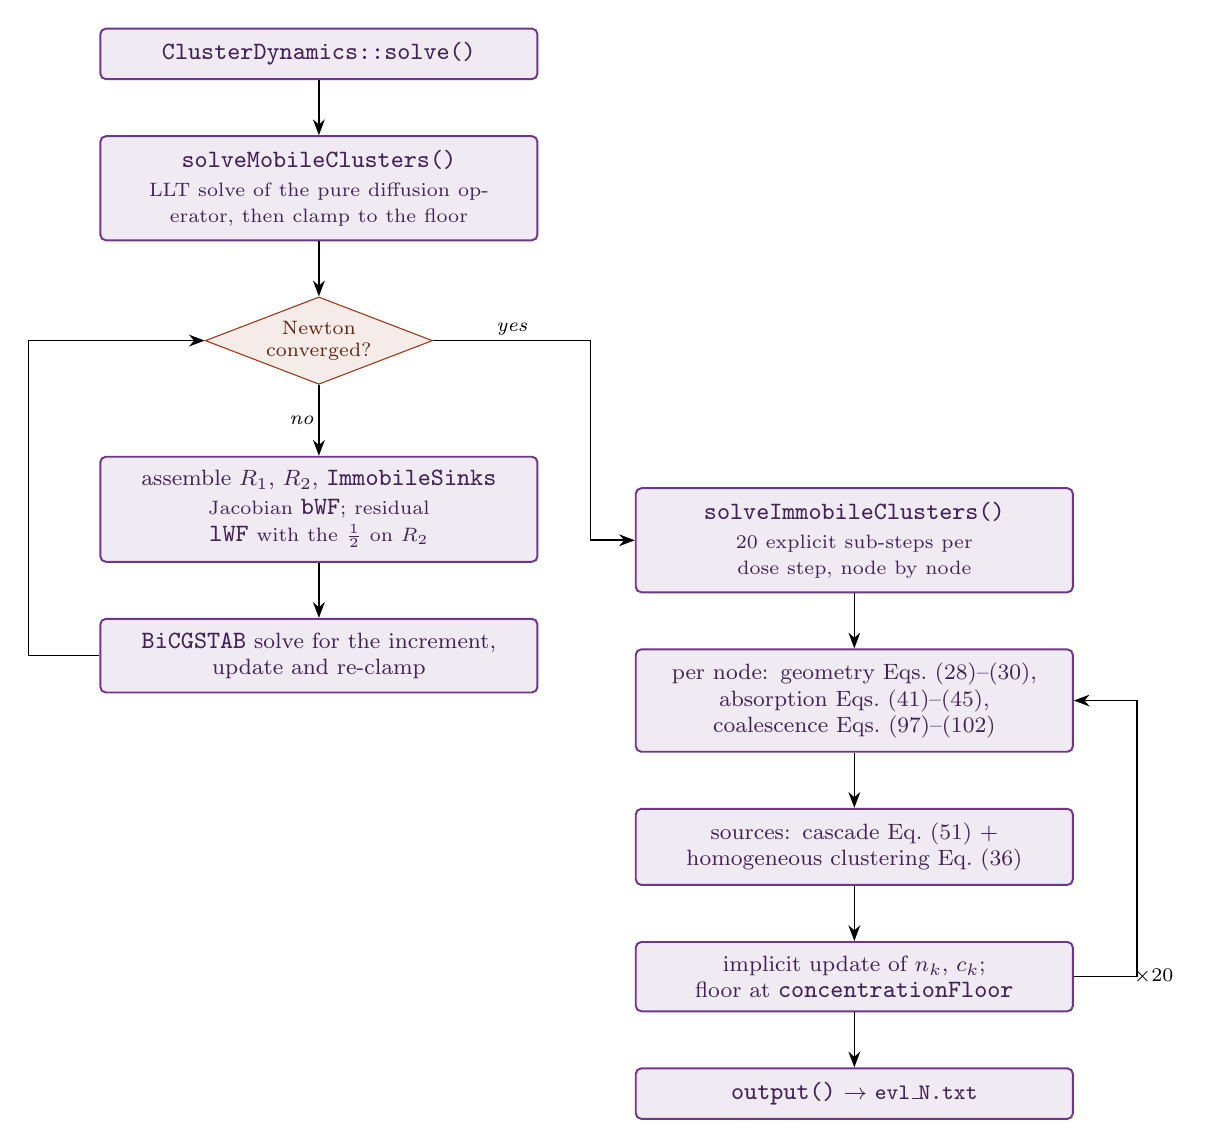
\begin{tikzpicture}[
  font=\footnotesize, node distance=7mm,
  stg/.style={draw, rounded corners=2pt, align=center, inner sep=5pt,
              text width=52mm, line width=0.7pt, fill=cMod!10, draw=cMod,
              text=cMod!60!black},
  dec/.style={draw, diamond, aspect=2.6, align=center, inner sep=1pt,
              fill=cCpp!10, draw=cCpp, text=cCpp!60!black, font=\scriptsize},
  a/.style={-{Stealth[length=2mm]}, line width=0.6pt},
  lbl/.style={font=\scriptsize\itshape, inner sep=1.5pt}
]
\node[stg] (s0) {\code{ClusterDynamics::solve()}};
\node[stg, below=of s0] (s1) {\code{solveMobileClusters()}\\[1pt]
  \scriptsize LLT solve of the pure diffusion operator, then clamp to the floor};
\node[dec, below=of s1] (d1) {Newton\\converged?};
\node[stg, below=9mm of d1] (s2) {assemble $R_1$, $R_2$, \code{ImmobileSinks}\\[1pt]
  \scriptsize Jacobian \code{bWF}; residual \code{lWF} with the $\tfrac12$ on $R_2$};
\node[stg, below=of s2] (s3) {\code{BiCGSTAB} solve for the increment,\\
  update and re-clamp};
\node[stg, below=13mm of d1, xshift=68mm] (s4) {\code{solveImmobileClusters()}\\[1pt]
  \scriptsize 20 explicit sub-steps per dose step, node by node};
\node[stg, below=of s4] (s5) {per node: geometry \drefs{28}{30},\\
  absorption \drefs{41}{45}, coalescence \drefs{97}{102}};
\node[stg, below=of s5] (s6) {sources: cascade \dref{51} $+$\\
  homogeneous clustering \dref{36}};
\node[stg, below=of s6] (s7) {implicit update of $n_k$, $c_k$;\\
  floor at \code{concentrationFloor}};
\node[stg, below=of s7] (s8) {\code{output()} $\rightarrow$ \file{evl\_N.txt}};

\draw[a] (s0) -- (s1);
\draw[a] (s1) -- (d1);
\draw[a] (d1) -- node[lbl,left]{no} (s2);
\draw[a] (s2) -- (s3);
\draw[a] (s3.west) -- ++(-9mm,0) |- (d1.west);
\draw[a] (d1.east) -- node[lbl,above]{yes} ++(20mm,0) |- (s4.west);
\draw[a] (s4) -- (s5);
\draw[a] (s5) -- (s6);
\draw[a] (s6) -- (s7);
\draw[a] (s7.east) -- ++(8mm,0) node[lbl,right,xshift=-1mm]{$\times 20$} |- (s5.east);
\draw[a] (s7) -- (s8);
\end{tikzpicture}
\caption{One dose step inside \MoD{}. The mobile Newton iteration runs to a
relative tolerance of $10^{-5}$; the immobile march then advances the loop
families against the converged, frozen mobile field. The linear losses
(coalescence, dissolution, emission) are integrated implicitly because their
coefficients times the sub-step exceed unity.}
\label{fig:inner}
\end{figure}

%==============================================================================
\section{Code Classes and Data Structures}
\label{sec:classes}

\subsection{The two state vectors}

Everything else follows from the choice of state.

\paragraph*{\ZrM{}: a flat array of length 19.}
Defined in \file{cpp\_utils/parameters.h} and mirrored in
\file{modelib\_coupling.py}; the layout is Table~\ref{tab:state0d}.

\begin{table}[htbp]
\centering
\caption{\ZrM{} state vector. \code{N\_PHYS}=12, \code{N\_ACC}=6,
\code{N\_RHO}=1, \code{N\_EQ}=19.}
\label{tab:state0d}
\begin{tabular}{@{}llll@{}}
\toprule
slice & contents & meaning & units \\
\midrule
\code{y[0:4]}   & $C_v, C_i, C_{2i}, C_{3i}$ & mobile species & atom fraction \\
\code{y[4:8]}   & $C_{iL}, C_{aiL}, C_{vL}, C_{avL}$ & loop number densities & per atom \\
\code{y[8:12]}  & $C_{iL}^{i}, C_{aiL}^{i}, C_{vL}^{v}, C_{avL}^{v}$ & loop contents & per atom \\
\code{y[12:18]} & six accumulators & conservation diagnostics & per atom \\
\code{y[18]}    & $\rho_N$ & evolving network density & m$^{-2}$ \\
\bottomrule
\end{tabular}
\end{table}

\noindent
The four loop families are the aligned/non-aligned split of the two loop types:
$iL$ and $aiL$ are prismatic \aloop{} interstitial loops, $vL$ and $avL$ basal
\cloop{} vacancy loops. The aligned fraction $f_a = (1+2f)/3$ carries the
stress-induced preferential nucleation of \dref{36}, where $f$ is the
stress-dependent alignment fraction. At zero applied stress $f=0$ and
$f_a = 1/3$, so the three prismatic variants are equivalent.

\begin{quote}\small
\textbf{Note.} The notebook declares \code{SIGMA\_N\_PA = 0.0} and records it in
the provenance manifest, but does \emph{not} route it into
\code{PARAMETER\_OVERRIDES}. The 0-D reference run therefore inherits the
workbook value $\sigma_n = 1\times10^{8}$~Pa, for which $f = 0.0518$ and
$f_a = 0.3679$ rather than $1/3$. The manifest and the run disagree on this one
quantity. It does not affect the \MoD{} side, which reads its stress state from
its own input files, nor the zero-stress verification of Route B; but a 0-D/3-D
comparison that assumes equivalent \aloop{} variants should add \code{sigma\_n}
to the override block.
\end{quote}

\paragraph*{\MoD{}: two finite-element trial functions.}
Defined in \file{ClusterDynamicsFEM.h}:
\begin{lstlisting}[language=C++]
typedef TrialFunction<'m',mSize,FiniteElementType> MobileTrialType;   // mSize=4
typedef TrialFunction<'i',iSize,FiniteElementType> ImmobileTrialType; // iSize=8
\end{lstlisting}
The degrees of freedom are laid out as \code{index = node*iSize + component},
with components $[0,n_F)$ the densities $n_k$ and $[n_F,2n_F)$ the contents
$c_k$, in family order $\{vL, a_1, a_2, a_3\}$. Note the family decomposition
differs from the 0-D: \MoD{} resolves the three crystallographically equivalent
\aloop{} prismatic variants explicitly, where the 0-D lumps them and splits by
alignment instead. \code{modelib\_export.py} performs the mapping.

\subsection{Python classes}

\paragraph*{\code{InputData} (\file{input\_data.py}).}
Owns three dictionaries --- \code{material\_params}, \code{physical\_props},
\code{model\_params} --- mirroring the workbook sheets, plus \code{derived},
which holds everything computed from them. The derived quantities are the
physics interface: jump frequencies
$\omega_m = z_c\nu_m\exp(-E^m_m/k_BT)$, equilibrium concentrations, the length
scales $\ell = z_c\Omega/(2\pi a^2)$, $\ell_a = \sqrt{\Omega/\pi b_a}$,
$\ell_c = \sqrt{\Omega/\pi b_c}$, the generation-rate partition
$G_v, G_i, G_{2i}, G_{3i}, G_{iL}, G_{aiL}, G_{vL}, G_{avL}$ satisfying
$\sum G_x = G$, and the DAD capture efficiencies $Z^{a}_{i}, Z^{a}_{v},
Z^{c}_{i}, Z^{c}_{v}$ of \drefs{63}{64}.

\paragraph*{\code{ReactionRates} (\file{reaction\_rates.py}).}
Holds no state of its own beyond a per-call cache. Its methods are the terms of
the master equation, named after the reaction they represent: \code{R\_i\_v},
\code{R\_i\_i}, \code{R\_i\_2i}, \code{R\_i\_3i}, \code{R\_2i\_2i},
\code{R\_2i\_3i} for the binary reactions; \code{R\_v\_s}, \code{R\_i\_s} for the
network sinks, built on the sink \emph{concentrations} of \dref{66},
$C^s_v = (a^2/z_c)\rho_N$ and $C^s_i = (a^2/z_c)Z_N\rho_N$;
\code{loop\_absorption} for \drefs{83}{89}; \code{flux\_v} and \code{flux\_i} for
the point-defect fluxes of \dref{41},
\begin{equation}
\phi_v = \omega_v c_v, \qquad
\phi_i = \omega_i\bigl(c_i + 2c_{2i} + 3c_{3i}\bigr);
\label{eq:fluxes}
\end{equation}
\code{nucleation\_rate\_*} for \dref{36}; \code{annealing\_rate\_*} for
\dref{38}; and \code{a\_shrink\_gate} for the smooth minimum-size gate of
\dref{91}.

\paragraph*{\code{RateEquations} (\file{rate\_equations.py}).}
Assembles those terms into $d\boldsymbol{y}/dt$. One method per equation
(\code{dCv\_dt}, \code{dCiL\_i\_dt}, \dots), plus \code{ode\_system} which
applies, in order: the positivity floor, the accumulator updates, the network
density source, a non-negativity guard that zeroes any derivative driving a
floored species further negative, and finally the \code{freeze\_mobile} branch
that zeroes \code{dydt[0:4]} --- \emph{last}, after every reaction term has
already read the mobile values. That ordering is what makes the operator split
exact rather than approximate.

\paragraph*{\code{MoDELibFEMSolver} (\file{modelib\_fem.py}).}
The adapter between the two codes. \code{write\_sink\_field()} converts the
per-family $(N, r)$ pairs into \MoD{} microstructure inputs, mapping the three
\aloop{} variants onto slip systems 6, 8, 10. \code{solve()} runs \code{DDomp}
and \code{\_read\_quadrature\_mobile\_field()} returns the mobile field at the
quadrature points. \code{available()} reports whether either \code{DDomp} or
\code{pyMoDELib} is built, which is what lets the notebook fall back to the
analytic placeholder rather than fail.

\subsection{C++ structures: \ZrM{}}

\paragraph*{\code{Parameters} (\file{cpp\_utils/parameters.h}).}
A flat aggregate of about 60 doubles, populated once from the command line so the
right-hand side performs arithmetic only --- no map lookups inside the integrator.
It carries the jump frequencies $\omega_i, \omega_v, \omega_{2i}$; the Boltzmann
factors $e_v = \exp(-E^F_v/k_BT)$, $e_{2i}$, $e_{3i}$ and the stress-modified
emission factors; the bias factors $Z_N, Z^a_i, Z^a_v, Z^c_i, Z^c_v$; the length
scales $\ell, \ell_a, \ell_c$; and the eight generation rates. The
\code{freeze\_mobile} flag also lives here.

\subsection{C++ classes: \MoD{}}

\paragraph*{\code{ClusterDynamicsParameters<dim>} (\file{ClusterDynamicsParameters.h}).}
Everything read from the material file, and every matrix derived from it. All
members are \code{const} and initialized in the constructor's member list, which
matters: C++ initializes members in \emph{declaration} order, and a member read
by another member's initializer must be declared first. (The \code{Eb} array was
declared after \code{R1} but read by \code{getR1()}, an uninitialized read that
silently dropped the Boltzmann factor from the cluster dissociation rates.) The
principal members are collected in Table~\ref{tab:cdp}.

\begin{table}[htbp]
\centering
\caption{Principal members of \code{ClusterDynamicsParameters}.}
\label{tab:cdp}
\begin{tabular}{@{}lll@{}}
\toprule
member & type & meaning \\
\midrule
\code{msVector} & $1\times4$ array & species sizes $\{-1,1,2,3\}$ \\
\code{D}, \code{invD}, \code{detD} & maps per grain & diffusion tensors, \dref{10} \\
\code{G} & $4\times1$ & effective production rates \\
\code{Eb} & $1\times4$ & binding energies, \dref{9} \\
\code{R1}, \code{R1cd} & $4\times4$ & first-order losses (sinks, dissociation) \\
\code{R2} & vector of $4\times4$ & binary reactions \\
\code{loopNucChannels} & map & clustering channels, \dref{36} \\
\code{immobileSpeciesVector} & $1\times4$ & family polarity \\
\code{immobileSpeciesBurgers} & $3\times4$ & Burgers directions, lattice components \\
\code{loopCascadeFractions} & $1\times4$ & $\varepsilon_k$, \dref{51} \\
\code{nNuc} & $1\times4$ & defects per cascade-nucleated loop, \dref{36} \\
\code{cLL}, \code{cLN} & $1\times4$ & coalescence coefficients, \dref{99} \\
\code{kappaLL}, \code{kappaLN} & double & Avrami overlap, \dref{98} \\
\code{tauVac} & double & vacancy-loop dissolution, \dref{95} \\
\code{dadAnisotropy}, \code{dadZ0} & $1\times4$ & $p_m$, $Z^0_m$ of \dref{15} \\
\code{loopSinkScale} & $1\times4$ & per-family sink calibration \\
\code{concentrationFloor} & double & positivity floor \\
\bottomrule
\end{tabular}
\end{table}

\noindent
Its methods build the derived objects: \code{getR1()} and \code{getR2()} assemble
the reaction matrices; \code{getLoopNucChannels()} selects the homogeneous
clustering channels of \dref{36}; \code{clusterRadius()} and
\code{clusterDensity()} implement the geometry of \drefs{28}{30}, interpolating
between the bi-pyramid law $\alpha_{bp}s_{bp}\pi r_{bp}n_{bp}$ of \dref{14} and
the planar loop law $2\pi r n$ of \drefs{12}{13} through the sigmoid of
\dref{30}; and \code{loopDADbias()} evaluates \dref{15},
\begin{equation}
Z^{\rm DAD,0}_{aL,m} = Z^{0}_{m}\,\frac{p_m + p_m^{-2}}{2},
\qquad
Z^{\rm DAD,0}_{cL,m} = Z^{0}_{m}\,p_m .
\label{eq:dad}
\end{equation}

\paragraph*{\code{ClusterDynamicsFEM<dim>} (\file{ClusterDynamicsFEM.h}).}
The numerical core. Its type aliases build the weak form compositionally from
MoDELib's expression templates: a trial function, its gradient, a flux matrix
applied to that gradient, a bilinear form pairing test and trial, and a weak form
integrating that bilinear form over the volume. Two linear solvers are held --- a
Cholesky solver \code{mSolver} for the pure diffusion operator, and a
BiCGSTAB-backed \code{rSolver} for the Newton system, both wrapped in
\code{FixedDirichletSolver} which eliminates the constrained degrees of freedom.

The public interface is four methods:
\code{solveMobileClusters()} (the Newton iteration on Eq.~\eqref{eq:mobile}),
\code{solveImmobileClusters()} (the pointwise dose march of \dref{34} and
\dref{39}), \code{clampMobileClusters()} (the positivity floor, exempting the
Dirichlet nodes), and \code{writeNodePositions()}.

\paragraph*{\code{EvalFunction} specializations.}
Three small classes supply the terms that depend on the local field, each
evaluated at quadrature points during assembly:

\begin{itemize}
\item \code{SecondOrderReaction} --- the binary block. For a pair $(a,b)$ it
holds $-K_{ab}$ in both symmetric slots, so that $\boldsymbol{c}^T R_2[a]
\boldsymbol{c} = -2K_{ab}c_a c_b$; the residual carries the compensating
$\tfrac12$ of \dref{1}, making the per-species loss rate $K_{ab}c_a c_b$.
\item \code{ImmobileSinks} --- the loop absorption sink acting on the mobile
species, $k^2_m = \sum_k Z(\text{type}(k),m)\,S_k$ from \drefs{11}{14}, returned
as $-k^2_m\bar{D}_m$ on the diagonal. The grain-boundary sink is deliberately
absent: unlike the 0-D reduction, which must lump it into a sink strength, the
spatially-resolved model captures it through the Dirichlet condition of
\dref{19}.
\item \code{FluxMatrix} and \code{InvDscaling} --- the diffusive flux
$-D\nabla c/\Omega$ and the symmetrizing test-function scaling.
\end{itemize}

\paragraph*{\code{ClusterDynamics<dim>} (\file{ClusterDynamics.h}).}
The outer wrapper: a \code{MicrostructureBase} subclass that plugs the
cluster-dynamics field into MoDELib's microstructure container. It owns the
parameters and the FEM object and implements the container interface ---
\code{solve()}, \code{getDt()}, \code{output()}, \code{updateConfiguration()} ---
together with the mechanical contributions (\code{averagePlasticDistortion},
\code{stress}, \code{inelasticDisplacementRate}) through which the cluster field
couples back to the elasticity solve.

\subsection{Relationships among the structures}

The dependency chain is short and strictly layered. In \MoD{}:
\begin{equation*}
\text{material file}
\;\longrightarrow\;
\code{ClusterDynamicsParameters}
\;\longrightarrow\;
\code{ClusterDynamicsFEM}
\;\longrightarrow\;
\{\code{SecondOrderReaction}, \code{ImmobileSinks}, \code{FluxMatrix}\}
\end{equation*}
with \code{ClusterDynamics} wrapping the FEM object and exposing it to
\code{DefectiveCrystal}. Nothing below the parameters object reads the material
file, and nothing above the FEM object touches degrees of freedom directly.

In \ZrM{} the corresponding chain is
\begin{equation*}
\text{workbook}
\;\longrightarrow\;
\code{InputData}
\;\longrightarrow\;
\code{ReactionRates}
\;\longrightarrow\;
\code{RateEquations}
\;\longrightarrow\;
\code{cpp\_bridge}
\;\longrightarrow\;
\code{Parameters}
\;\longrightarrow\;
\text{RHS},
\end{equation*}
where the Python and C++ right-hand sides are deliberate mirrors: the Python one
is the readable reference, the C++ one the production integrator, and they are
required to agree.

The two chains meet only at \code{modelib\_coupling} and \code{modelib\_fem} in
Route A, and only through the material definitions in Route B. That is the whole
of the coupling surface, and keeping it that small is what has allowed the two
codes to be reconciled term by term.

%==============================================================================
\section{Changes and Differences from Upstream}
\label{sec:changes}

Everything described so far is the architecture of \Zrd{}, the branch. This
section separates what was inherited from upstream from what was added, so
that the preceding sections are not read as a description of the upstream code.

\subsection{Which upstream --- a correction}
\label{sec:whichupstream}

Earlier revisions of this document compared \Zrd{} against \file{main} of
\MoDnnl{}. Those statements are individually accurate --- a checkout confirms
every row of Table~\ref{tab:upstream} --- but \MoDnnl{} is the wrong baseline
for cluster dynamics, and comparing against it makes the immobile solver look
like an invention from nothing. It is not.

\begin{table}[htbp]
\centering
\caption{The two upstream repositories. Both were checked out and read.}
\label{tab:twoupstream}
\begin{tabular}{@{}lcp{0.52\textwidth}@{}}
\toprule
repository & \code{iSize} & immobile machinery \\
\midrule
\file{mlm335/MoDELib2-NNL}  & 0 &
  none: empty \code{solveImmobileClusters()}, no \file{ImmobileSinkRate.h} or
  \file{SpatialODESolver.h}, and a literal \code{// Missing immobile sinks}
  placeholder \\
\file{mlm335/MoDELib-fullCD} & 8 &
  complete: \file{ImmobileSinkRate.h}, \file{SpatialODESolver.h},
  \file{FirstOrderReaction.h}, and continuum-to-discrete loop conversion \\
\bottomrule
\end{tabular}
\end{table}

\noindent
\textbf{\MoDfull{} is the correct baseline.} Measured against it, \Zrd{}'s
immobile solver is a \emph{re-discretization} of an existing scheme: 31
cluster-dynamics parameter keys are shared verbatim, and most of the remainder
are renames (\code{loopNucDefects}$\to$\code{nNuc},
\code{loopCoalLL/LN}$\to$\code{cLL/cLN},
\code{loopAnnealTau0\_SI}$\to$\code{tau0\_vLoop\_SI},
\code{loopCoalNetwork\_SI}$\to$\code{rhoNetwork\_SI},
\code{minimumLoopSize}$\to$\code{r\_min}). What differs is how the same physics
is discretized:

\begin{table}[htbp]
\centering
\caption{Immobile discretization, \MoDfull{} against \Zrd{}.}
\label{tab:fullcdvsours}
\begin{tabular}{@{}lp{0.33\textwidth}p{0.33\textwidth}@{}}
\toprule
 & \MoDfull{} & \Zrd{} \\
\midrule
rate & Galerkin: assembled at quadrature points, then $L^2$-projected through
       the consistent mass matrix (CG to $10^{-4}$) & nodal collocation; no
       mass matrix \\
time update & explicit Euler, then \emph{sequential} implicit loss factors
       $(1+\mathrm dt\lambda_k)^{-1}$ per channel & one \emph{fused}
       semi-implicit update \\
sub-cycling & none, one step of \code{dtMax} & \code{nSub}$=20$ per dose step \\
\bottomrule
\end{tabular}
\end{table}

\noindent
Genuinely new in \Zrd{}: \code{dadAnisotropy}/\code{dadZ0} (DAD reconciliation
with the 0-D), \code{atomicVolume\_SI}, \code{concentrationFloor},
\code{loopSinkScale}, size-dependent vacancy-loop emission, and the bi-pyramid
family. Genuinely \emph{lost}: \code{clusterDiscretizationTime} and
\code{initializeDiscreteClimbLoops()}. \MoDfull{} converts its continuum loop
field into discrete climb loops once the dose passes a threshold; \Zrd{} has no
such transition, which is the largest functional regression of the fork and the
capability its name refers to.

Note also that \file{Zr4.txt} in this checkout carries no immobile keys, but
that is a property of one file and not evidence about upstream: \MoDfull{}'s
\file{Zr4\_Fitted.txt} and \file{Zr4\_BMD19\_nuc.txt} each carry the full
sixteen-key immobile set.

\subsection{What \MoDnnl{} contains}

The remainder of this section is stated against \MoDnnl{}, and is retained
because it is the accurate account of \emph{that} repository and of how much of
the model had to be written on this branch without reference to \MoDfull{}
(Table~\ref{tab:upstream}). Read it as the difference from the
\emph{dislocation-dynamics} upstream, not from the cluster-dynamics one.

\begin{table}[htbp]
\centering
\caption{State of the immobile (loop) machinery in \MoDnnl{}.}
\label{tab:upstream}
\begin{tabular}{@{}ll@{}}
\toprule
item & state on \MoDnnl{} \file{main} \\
\midrule
\code{iSize} & $0$ --- no immobile species exist \\
\code{solveImmobileClusters()} & present, but an \emph{empty function body} \\
\code{ImmobileSinks.h} & does not exist \\
mobile solve & carries the comment \code{// Missing immobile sinks} \\
\file{Zr4.txt} immobile block & absent; the file ends at \code{otherSinks\_SI=0.0 0.0 0.0 0.0;} \\
\bottomrule
\end{tabular}
\end{table}

\noindent
\MoDnnl{} therefore solves the mobile steady-state PDE of \dref{1} --- and
nothing else. Diffusion, cascade production, the first-order losses $R_1$ and the
binary reactions $R_2$ are all present and working. \emph{The entire immobile
half of the model, deliverable Sec.~2.2, was not implemented.}

Some scaffolding for it did exist. The geometry helpers
\code{clusterRadius()}, \code{clusterDensity()}, \code{sigmoid()},
\code{rpyr()} and \code{rloop()} --- \drefs{28}{30} --- are all upstream code.
With \code{iSize=0}, however, nothing ever called them.

\subsection{Equations added}

Table~\ref{tab:eqadded} lists the physics that had no upstream implementation,
against the equation of the deliverable that each term realizes.

\begin{table}[htbp]
\centering
\caption{Physics with no implementation in \MoDnnl{}. All of it is new on the
\file{zr3d\_ghoniem} branch --- though \MoDfull{} implements most of it too, by
the different discretization of Table~\ref{tab:fullcdvsours}.}
\label{tab:eqadded}
\begin{tabular}{@{}llp{0.36\textwidth}@{}}
\toprule
equation & content & implemented in \\
\midrule
\dref{34} & loop density: nucleation $-$ coalescence $-$ dissolution &
  \code{solveImmobileClusters()} \\
\dref{39} & loop content: cascade seed $+$ absorption $-$ coalescence
  $-$ annealing $-$ emission & \code{solveImmobileClusters()} \\
\dref{36} & homogeneous SIA clustering nucleation $\Phi_{\rm clus}$ &
  \code{getLoopNucChannels()} \\
\drefs{11}{14} & loop absorption sink on the mobile species &
  \code{ImmobileSinks.h} (new file) \\
\dref{15} & DAD capture efficiencies from $p_m$, $Z^0_m$ &
  \code{loopDADbias()} (new method) \\
\drefs{41}{45} & absorption fluxes with the $|m_m|$ cluster weighting &
  \code{solveImmobileClusters()} \\
\dref{91} & minimum-stable-size gate on the shrinking channel &
  \code{solveImmobileClusters()} \\
\dref{95} & vacancy-loop dissolution &
  \code{solveImmobileClusters()} \\
\drefs{54}{56} & size-dependent thermal vacancy emission &
  \code{solveImmobileClusters()} \\
\drefs{97}{102} & Avrami coalescence, two channels &
  \code{solveImmobileClusters()} \\
\bottomrule
\end{tabular}
\end{table}

\noindent
Two of these deserve a note on \emph{how} they were added rather than merely
that they were.

\paragraph*{The loop absorption sink.} \code{ImmobileSinks} is written as an
\code{EvalFunction} mirroring the existing \code{SecondOrderReaction}, so it
assembles into the mobile Newton system through the same mechanism as every
other reaction term --- \code{bWF\_RI} into the Jacobian, \code{lWF\_RI} into the
residual. The sink set is the 0-D one \emph{except} the grain boundary, which is
imposed spatially by the Dirichlet condition of \dref{19} and would otherwise be
counted twice. The network dislocation sink required no new code: it reuses the
existing \code{otherSinks\_SI} plumbing, which upstream was simply set to zero.

\paragraph*{The clustering nucleation source.} Rather than being posited
separately, $\Phi_{\rm clus}$ is read off the reaction network the mobile solve
already uses, so that the loops gain exactly what the mobile field loses.
\code{getLoopNucChannels()} selects the pairs $(a,b)$ whose reactants share
polarity and whose product size $m_a+m_b$ is carried by no mobile species --- the
products that fall off the end of the truncated cluster ladder. For
$\{v,i,2i,3i\}$ this selects $i+3i$, $2i+2i$ and $2i+3i$. Those interstitials
were previously unaccounted for: \code{getR2()} debits the reactants and credits
nothing, which is the origin of the \code{Warning: Sum of R2 is not zero} message
at start-up.

\subsection{Corrections to pre-existing code}

Four defects were found in code that was already there. They are listed
separately from the additions because they affect the original code as
distributed.

\begin{description}
\item[Binding energies read before initialization.]
\code{getR1()} reads the binding-energy array \code{Eb} to build the cluster
dissociation rates, but \code{Eb} was declared \emph{after} \code{R1} in the
class. C++ initializes members in declaration order, not in the order of the
constructor's initializer list, so this was an uninitialized read: the Boltzmann
factor $\exp(-E_b/k_BT)$ evaluated to unity instead of $3.8\times10^{-9}$,
inflating the dissociation rate to the bare attempt frequency and suppressing
$C_{2i}$ and $C_{3i}$ by a factor $2.4\times10^{6}$.
\textbf{This is a defect of the original code, not of the present work.} It was
invisible in the distributed calibration because every \code{Eb\_eV} was set to
5~eV, for which $\exp(-5/k_BT)\sim10^{-44}$ is negligible whether or not the
factor is applied. Giving the di-interstitial its physical $0.957$~eV is what
exposed it. \emph{It should be reported upstream}: it affects any \MoD{} run
with a non-negligible cluster binding energy.

\item[The diffusion operator was scaled relative to the reactions.]
\code{FluxMatrix} divides $D$ by \code{cdp.omega}, and the weak form multiplied
the flux back by \code{ddBase.poly.Omega}. The two were the same quantity until
the cluster-dynamics atomic volume became independently settable, after which
the entire diffusion operator carried a spurious factor of
\code{poly.Omega/cdp.omega} $= 3.98$ relative to every reaction term.

\item[The minimum stable radius was never converted from metres.]
\code{r\_min} is given in metres in the material file but compared against radii
expressed in units of $b$, leaving the gate of \dref{91} permanently open.

\item[The atomic volume was the lattice \emph{cell} volume.]
The polycrystal class returns $\det(\text{lattice basis})$. For a hexagonal
lattice that cell contains two atoms, so the quantity is not the atomic volume
the cluster-dynamics equations assume, and every content--radius--density
conversion inherited the error. An optional material-file key,
\code{atomicVolume\_SI}, now supplies it explicitly, falling back to the previous
behaviour when absent.
\end{description}

\subsection{Input data: the mobile block}

Po's \file{Zr4.txt} is left untouched --- \file{main} still runs his standalone
calibration unchanged. The reconciled definition is the separate file
\file{Zr3d\_ghoniem.txt}, whose mobile block resets seven keys and adds one
(Table~\ref{tab:mobdiff}).

\begin{table}[htbp]
\centering
\caption{Mobile-species parameters: original against reconciled.}
\label{tab:mobdiff}
\begin{tabular}{@{}p{0.30\textwidth}p{0.31\textwidth}p{0.31\textwidth}@{}}
\toprule
key & \file{Zr4.txt} (original) & \file{Zr3d\_ghoniem.txt} \\
\midrule
\code{mobileSpeciesSurviving} \code{Efficiency} & \code{0.01} & \code{1.0} \\
\code{mobileSpeciesCascade} \code{Fractions} &
  \code{1.0 0.6 0.3212 0.0788} &
  \code{0.995 0.97788714 0.005 0.00333333} \\
\code{mobileSpeciesEnergy} \code{Formation\_eV} &
  \code{1.5 3.0 6.0 8.0} & \code{1.6 3.0 6.0 8.0} \\
\code{mobileSpeciesEnergy} \code{Migration\_eV} &
  $0.9$ (v), $0.09$ (i), $0.041$--$0.187$ (2i, 3i); anisotropic &
  $1.2$ (v), $0.759101$ (i, 2i, 3i); isotropic \\
\code{mobileSpeciesD0\_SI} &
  \code{4.9639e-10} (v), \code{8.1882e-10} (i, 2i, 3i) &
  \code{5.21645e-7}, all species \\
\code{reactionPrefactorMap} &
  \code{2.856} for v$+$i, \code{1.0} or \code{0.0} elsewhere; $2i+2i$ and
  $2i+3i$ switched off &
  ten values derived from the 0-D jump frequencies; $2i+2i$ and $2i+3i$
  switched on \\
\code{otherSinks\_SI} & \code{0.0 0.0 0.0 0.0} &
  \code{1.88e14}, \code{1.8988e14}$\times3$ \\
\code{atomicVolume\_SI} & \emph{key did not exist} & \code{1.2e-29} \\
\bottomrule
\end{tabular}
\end{table}

\noindent
Three of these are worth quantifying. The original migration energies give
$D_i$ about $1200\times$ and $D_{2i}$ about $2.5\times10^{8}\times$ the 0-D
values at 573~K. The original \code{otherSinks\_SI=0} means there is
\emph{no network dislocation sink at all}. And the original
\code{mobileSpeciesCascadeFractions} do not partition the displacement rate the
way the 0-D does: the reconciled values enforce
$G_v + G_i + G_{2i} + G_{3i} + G_{iL} + G_{aiL} + G_{vL} + G_{avL} = G$.

The reaction prefactors are the one place where the two codes had to be made to
agree algebraically rather than by substitution. \MoD{} forms
$K_{ab} = p_{ab}\,4\pi(r_a+r_b)(D_a+D_b)/\Omega$ while \ZrM{} forms
$K_{ab} = f_{ab}(\omega_a+\omega_b) = f_{ab}(z_c/a^2)(D_a+D_b)$, so
\begin{equation}
p_{ab} = f_{ab}\,\frac{z_c}{a^2}\,\frac{\Omega}{4\pi(r_a+r_b)} ,
\label{eq:prefactor}
\end{equation}
with $f_{ab} = 0.5$ for v$+$i (the 0-D recombination factor) and unity
otherwise. Pairs involving $2i$ or $3i$ additionally carry the ratio of
diffusivities that restores the $\omega_{2i}$-based 0-D rate, because those
species transport at the monomer diffusivity here.

\subsection{Input data: the immobile block}

There is no ``before'' column for this one: the twenty-odd keys of
Table~\ref{tab:immdiff} are all new, because none of the immobile machinery
existed.

\begin{table}[htbp]
\centering
\caption{Immobile-species keys, all added. None has a counterpart in
\file{Zr4.txt}.}
\label{tab:immdiff}
\begin{tabular}{@{}lp{0.60\textwidth}@{}}
\toprule
group & keys \\
\midrule
family definition &
  \code{immobileSpeciesVector}, \code{immobileSpeciesRelRelaxVol},
  \code{immobileSpeciesBurgers} \\
nucleation &
  \code{loopCascadeFractions} ($\varepsilon_k$), \code{nNuc} ($n^{\rm nuc}_k$),
  \code{evc}, \code{Nvmax} \\
geometry &
  \code{alpha\_bp}, \code{delVPyramid}, \code{w0}, \code{n\_s},
  \code{nmin}, \code{nmax}, \code{r\_min} \\
coalescence &
  \code{cLL}, \code{cLN}, \code{kappaLL}, \code{kappaLN} \\
dissolution and emission &
  \code{tau0\_vLoop\_SI}, \code{Ea\_vLoop\_eV}, \code{Eb\_eV} \\
sinks and bias &
  \code{rhoNetwork\_SI}, \code{dadAnisotropy}, \code{dadZ0},
  \code{loopSinkScale} \\
numerics &
  \code{concentrationFloor} \\
\bottomrule
\end{tabular}
\end{table}

\noindent
Two of these are calibration choices rather than physical constants, and are
flagged here because they are easy to mistake for the latter.

\code{loopSinkScale} reproduces \ZrM{}'s sink convention exactly. The 0-D applies
the \cloop{} radius prefactor $\ell_c = \sqrt{\Omega/\pi b_c}$ to \emph{all four}
families --- $\ell_a$ is computed and never used --- whereas the 3-D builds
$r_k$ from each family's own $|b_k|$. Each family therefore needs
$\sqrt{|b_k|_{\rm 3D}/b_c^{\rm 0D}}$, and the \cloop{} channel additionally
carries the fitted $Q = 0.287931$. Setting all four to unity recovers the purely
geometric form.

\code{dadAnisotropy} and \code{dadZ0} are fitted, not derived. They are obtained
by closed-form inversion of \dref{15} against the 0-D symmetric forms
\drefs{63}{64}, exactly, to a residual of $10^{-16}$. The cost is that the fitted
$p_m$ is \emph{not} the anisotropy the migration tensors imply, so these runs do
not exercise the tensorial-DAD mechanism that is the distinctive physics of the
3-D model; \dref{15} is acting as a two-parameter fitting form. The fit is also
tied to $T=573$~K, because $\delta_i$ is temperature-interpolated in the 0-D.

\subsection{What is unchanged}

Of the eighteen files that differ from \file{main}, most are additions. Nothing
outside the cluster-dynamics path was touched: elasticity, mobility laws,
gamma-surface, the discrete-dislocation machinery, the mesh and FEM
infrastructure, and the microstructure generator are all as distributed. Within
the cluster-dynamics path, the mobile transport operator, the $R_1$ and $R_2$
assembly, the trial-function and weak-form types, and the linear solvers are
Po's --- the changes to them are the four corrections above, not redesigns.

Two files in the branch are \emph{not} intended for upstream:
\file{CMakeLists.txt} and \file{tools/CMakeLists.txt} carry local-environment
adaptations (Eigen include path moved from MacPorts to a Linux location, the
maintainer's Qt path removed, and the \code{DDqt} target disabled because Qt is
absent here). They are correct for a Linux or WSL build and would break a macOS
build, and should be dropped from any pull request.

%==============================================================================
\appendix
\section{Code Manual}
\label{sec:manual}

This appendix is operational: what to install, what to run, what to change, and
what to check when something goes wrong.

\subsection{Prerequisites}

\begin{table}[htbp]
\centering
\caption{Environment.}
\label{tab:env}
\begin{tabular}{@{}lll@{}}
\toprule
component & version & note \\
\midrule
Python & 3.14 & virtual environment \file{Fluor\_Zr/.Zr\_venv/} \\
Jupyter kernel & \code{fluor\_zr} & registered as ``Python 3.14 (Fluor\_Zr)'' \\
SUNDIALS & 7.1.1 & \file{Libraries/sundials-7.1.1/}; CVODE and ARKODE \\
CMake & $\ge 3.16$, $< 4$ & CMake 4 rejects \code{cmake\_minimum\_required(3.1)} \\
Eigen & 3.4 & \MoD{} dependency \\
FFTW & 3 & \code{libfftw3-dev}; \MoD{} will not configure without it \\
compiler & C++17 / C++20 & \ZrM{} needs C++17, \MoD{} needs C++20 \\
\bottomrule
\end{tabular}
\end{table}

\noindent
\textbf{Do not use Anaconda Python} for this project: its NumPy conflicts with
the SciPy build in the virtual environment.

On Windows, \MoD{} is built and run inside WSL. Its \code{DDomp} is a Linux ELF
and is invoked through \code{wsl.exe}, with Windows paths translated to
\file{/mnt/<drive>/...}. \ZrM{} builds natively on Windows.

\subsection{Building}

\paragraph*{\ZrM{} C++ solver.}
\begin{lstlisting}
cd ZrMicro/cpp_utils
cmake -S . -B ../build -DCMAKE_BUILD_TYPE=Release
cmake --build ../build --config Release
\end{lstlisting}
Use \code{Release}: the parameter fit calls the solver thousands of times, and
the OpenMP batch mode is only worth having when optimized. CMake auto-detects
OpenMP; the build still works serially without it.

\paragraph*{\MoD{}.}
\begin{lstlisting}
cd <DisloCluster>/MoDELib3/build
cmake -S .. -B . -DCMAKE_BUILD_TYPE=Release
cmake --build . --target DDomp -j 12
\end{lstlisting}
The build takes 10--30 minutes from clean. Two files on the \file{zr3d\_ghoniem}
branch are local-environment adaptations and would break a macOS build:
\file{CMakeLists.txt} (Eigen path, Qt path removed) and
\file{tools/CMakeLists.txt} (\code{DDqt} disabled). Drop both from any pull
request to upstream.

\subsection{Running}

\paragraph*{Route A --- coupled march.}
Open \file{ZrMicro/code/coupled\_0d\_3d\_ZrMicro.ipynb} on the
\code{dislocluster} kernel and run all cells; or headless:
\begin{lstlisting}
.DisloClusterVenv\Scripts\python.exe -m nbconvert --to notebook --execute \
    --ExecutePreprocessor.kernel_name=dislocluster \
    ZrMicro/code/coupled_0d_3d_ZrMicro.ipynb
\end{lstlisting}
Everything the user is expected to change is in cell 12. Before the first
coupled run the simulation directory must be seeded once:
\code{seed\_sim\_dir\_from\_tutorial(MODELIB\_ROOT, SIM\_DIR)}, then run its
\file{generateInputFiles.py}. Until that is done the notebook silently falls
back to the analytic placeholder --- it says so loudly in its output, and that
message should be read every time.

\paragraph*{Route B --- monolithic \MoD{} run.}
\begin{lstlisting}
cd <DisloCluster>/MoDELib3/tutorials/zrmicro_coupled
./clean_run.sh
\end{lstlisting}
The script refreshes the material file and the mesh from \file{Library/}
(LF-converted), regenerates \file{evl\_0}, then runs
\code{microstructureGenerator} and \code{DDomp}. A 31-step run to 30~dpa takes
about one hour on 24 cores. Output appears in \file{evl/} as
\file{evl\_N.txt} plus \file{cdNodes.txt}.

\paragraph*{0-D only.}
\file{ZrMicro/code/ZrMicro.ipynb} runs the 0-D model alone and produces the full
figure suite plus \file{provenance.md} in a timestamped output directory.

\subsection{Post-processing}

\begin{lstlisting}
from py_utils.modelib_fields import plot_field_panels
from py_utils import modelib_gb as gb

plot_field_panels(EVL, steps=[0,4,9,29], doses=[1,5,10,30],
                  species=("Cv","Ci","C2i","C3i"), out_file=...)
gb.plot_density_profiles(EVL, steps, doses, max_nm=150.0, n_bins=45,
                         out_file=...)
\end{lstlisting}
Output is written \emph{after} \code{solve()}, so \file{evl\_N} holds the state
at $N+1$ dose steps --- \file{evl\_0} is 1~dpa, not 0. Loop diameters must be
formed from binned mean content and density, never by averaging nodal
diameters: size is a ratio of two fields, and the mean of a ratio is not the
ratio of the means.

\subsection{Changing things}

\begin{table}[htbp]
\centering
\caption{Where to change what.}
\label{tab:whereto}
\begin{tabular}{@{}p{0.34\textwidth}p{0.60\textwidth}@{}}
\toprule
to change & edit \\
\midrule
irradiation conditions ($T$, $G$, $\sigma$) &
  cell 12 of the notebook \emph{and} \file{polycrystal.txt} /
  \file{Zr3d\_ghoniem.txt}; they are not linked \\
0-D material parameters &
  the workbook, or \code{PARAMETER\_OVERRIDES} (which wins) \\
3-D material parameters &
  \file{Library/Materials/Zr3d\_ghoniem.txt}, then re-run
  \file{clean\_run.sh} so the copy in \file{inputFiles/} is refreshed \\
dose schedule (Route A) &
  \code{DOSE\_START}, \code{DOSE\_INTERVAL}, \code{DOSE\_MAX} \\
dose schedule (Route B) &
  \code{Nsteps} and \code{dtMax} in \file{DD.txt} \\
mesh or domain size &
  \code{meshFile} and \code{F} in \file{polycrystal.txt} \\
number of loop families &
  \code{iSize} in \file{ClusterDynamicsParameters.h}, plus every
  \code{1,iSize/2} array in the material file \\
0-D solver method &
  \code{solver\_method} in \code{SOLVER\_CONFIG}; CVODE BDF + dense is the
  recommended default \\
\bottomrule
\end{tabular}
\end{table}

\noindent
Note that the temperature appears in \emph{three} places --- the workbook, the
notebook override, and \file{polycrystal.txt} --- and that
\code{dadAnisotropy}/\code{dadZ0} are fitted at 573~K. Changing $T$ requires
refitting them, or the DAD bias will be silently wrong.

\subsection{Troubleshooting}

\begin{quote}\small
\textbf{The governing rule of this stack: almost every failure exits zero.}
The \MoD{} build script, \code{DDomp} with a missing \file{evl\_0}, a missing
material key, a CRLF mesh, and several solver failures all return status 0.
Verify by artifacts on disk and by log tails, never by exit status.
\end{quote}

\begin{longtable}{@{}p{0.36\textwidth}p{0.58\textwidth}@{}}
\caption{Symptoms and causes.}
\label{tab:trouble}\\
\toprule
symptom & cause and fix \\
\midrule
\endfirsthead
\toprule
symptom & cause and fix \\
\midrule
\endhead
\code{microstructureGenerator} never terminates &
  It is the discrete-dislocation path, inserting loops one at a time; CD loop
  densities need $\sim10^{11}$ of them. Set \code{useDislocations=0} and
  \code{targetDensity=0}. \\
Loop content comes out at exactly $3\times$ the expected value &
  \code{startAtTimeStep=-1} resumed from a stale \file{evl\_N} and
  double-counted dose. Pin \code{startAtTimeStep=0}. \\
Parser reports zero mesh nodes, no error &
  CRLF line endings in the \file{.msh}. \file{clean\_run.sh} LF-converts it on
  every run for this reason. \\
Newton residual stalls near $10^{5}$ &
  An initial-guess problem, not a linear-algebra one. The direct
  \code{SparseLU} branch was tried and fails in \code{compute()} on the
  $\sim$96k-dof matrix; the iterative branch is the working one. \\
Run restarts from the previous dose &
  \file{evl\_0.txt} is both the initial configuration and the runID~0 output.
  Regenerate it every run. \\
Notebook silently produces analytic profiles &
  The fast-solve backend fell back to \code{placeholder}. Check whether
  \code{DDomp} is built and \file{SIM\_DIR/inputFiles/} is seeded. \\
$C_{2i}$, $C_{3i}$ orders of magnitude low &
  Historically the \code{Eb}-before-\code{R1} declaration-order bug. Fixed on
  this branch; if it reappears, check that no member's initializer reads a
  member declared after it. \\
Three \aloop{} families give different densities at zero stress &
  Burgers vectors supplied in Cartesian rather than lattice components. The
  zero-stress symmetry check is the fastest detector of this class of error. \\
\bottomrule
\end{longtable}

\subsection{Reproducibility}

Every run writes a timestamped, git-tagged directory
\file{output/<YYYYMMDD\_HHMMSS>\_<git-hash>/} containing the figures and
\file{provenance.md}, the latter recording every input parameter, the software
environment, and the solver statistics. The 0-D reference used throughout this
work is \file{output/20260622\_144021\_7959445}.

One caution on reproducing it: \file{provenance.md} stores values to four
significant figures only, so re-reading it will \emph{not} reproduce the run.
The full-precision fitted set lives in the \code{PARAMETER\_OVERRIDES} block of
the notebook, which is why that block is pinned rather than inherited from the
workbook.

\end{document}
